% !TEX encoding = UTF-8 Unicode
\documentclass{beamer}
\usetheme{Szeged}

\usepackage{color}
\usepackage{url}
\usepackage[utf8]{inputenc}
\usepackage{graphicx}

\usepackage[english, serbian]{babel}

%\usepackage[unicode]{hyperref}
\usepackage{amsmath}
\usepackage{amsthm}
\usepackage{amssymb}
\hypersetup{colorlinks,citecolor=green,filecolor=green,linkcolor=blue,urlcolor=blue}
\usepackage[title]{appendix}
\usepackage{float}
\usepackage[graphicx]{realboxes}
\usepackage{chngcntr}
\counterwithin{figure}{section}
\usepackage{listings}
\usepackage{textcomp}
\usepackage{xcolor}
\usepackage{adjustbox}
\lstset {
    language=Java,
    frame=none,
    %xleftmargin=-.25in,
    %xrightmargin=.25in
    framesep=10pt,
    tabsize=4,
    showstringspaces=false,
    upquote=true,
    commentstyle=\color{gray},
    keywordstyle=\color{orange},
    stringstyle=\color{red},
    basicstyle=\scriptsize\ttfamily,
    emph={int,char,double,float,unsigned,void,bool},
    emphstyle={\color{blue}},
    escapechar=\&,
    classoffset=1,
    morekeywords={>,<,.,;,,,-,!,=,~},
    keywordstyle=\color{weborange},
    classoffset=0,
    breaklines=true
}

\usepackage[font=scriptsize,labelfont=bf]{caption}


\title{Sinteza popravki programa na osnovu ispravnih primera}

\author{\href{mailto:mi14031@matf.bg.ac.rs}{Ivan Ristović}, \href{mailto:mi14042@matf.bg.ac.rs}{Milana Kovačević}, \href{mailto:mi14207@matf.bg.ac.rs}{Strahinja Stanojević}
}
\date{septembar 2018.}


\begin{document}
\begin{frame}
    \titlepage
\end{frame}

\begin{frame}{Zadatak}
    \begin{itemize}
        \item Ulaz: Dva ise\v{c}ka koda, jedan koji slu\v{z}i kao specifikacija i drugi sa gre\v{s}kama
        \item Zadatak: ispraviti kod da postane semanti\v{c}ki ekvivalentan ispravom kodu
        \item Ispravljen kod treba da zadrzi originalnu strukturu sto je vi\v{s}e mogu\'c{}e
    \end{itemize}
\end{frame}


\begin{frame}[fragile]{Primeri ulaza}
\begin{figure}[!h]
\centering
\begin{tabular}{ p{4.5cm} p{4.5cm} }
\begin{lstlisting}
int foo1()
{
    int x = 1, a = 2;
    return x + a;
}
\end{lstlisting}
&
\begin{lstlisting}
int foo2()
{
    int x = 0, a = 2;
    return x + a;
}
\end{lstlisting}
\end{tabular}
\end{figure}
\end{frame}


\begin{frame}[fragile]{Primeri ulaza}
    \begin{itemize}
        \item Ekvivalentno?
    \end{itemize}
\begin{figure}[!h]
\centering
\begin{tabular}{ p{4.5cm} p{4.5cm} }
\begin{lstlisting}
int fooEq1()
{
    int x = 1;
    int a = 2;
    return x + a + 1;
}
\end{lstlisting}
&
\begin{lstlisting}
int fooEq2()
{
    return 4;
}
\end{lstlisting}
\end{tabular}
\end{figure}
\end{frame}


\begin{frame}[fragile]{Primeri ulaza}
    \begin{itemize}
        \item Sporedni efekti
    \end{itemize}
\begin{figure}[!h]
\centering
\begin{tabular}{ p{4.5cm} p{4.5cm} }
\begin{lstlisting}
int fooSideEff()
{
    print("Hello!");
    return 1;
}
\end{lstlisting}
&
\begin{lstlisting}
int foo()
{
    return 1;
}
\end{lstlisting}
\end{tabular}
\end{figure}
\end{frame}

\begin{frame}[fragile]{Primeri ulaza}
    \begin{itemize}
        \item Mogu\'c{}e evaluirati u nekim slu\v{c}ajevima
    \end{itemize}
\begin{figure}[!h]
\centering
\begin{tabular}{ p{4.5cm} p{4.5cm} }
\begin{lstlisting}
int anotherFooEq1()
{
    int x = 0;
    x += 3;
    return x;
}
\end{lstlisting}
&
\begin{lstlisting}
int anotherFooEq2()
{
    int a = 0;
    a++;
    a++;
    ++a;
    return a;
}
\end{lstlisting}
\end{tabular}
\end{figure}
\end{frame}


\begin{frame}[fragile]{Primeri ulaza}
\begin{figure}[!h]
\centering
\begin{tabular}{ p{4.5cm} p{4.5cm} }
\begin{lstlisting}
int ambFoo1(int x)
{
    if (x >= 0)
        return 1;
    else
        return 0;
}
\end{lstlisting}
&
\begin{lstlisting}
int ambFoo2(int y)
{
    return y % 2;
}
\end{lstlisting}
\end{tabular}
\end{figure}

\begin{figure}[!h]
\centering
\begin{tabular}{ p{4.5cm} p{4.5cm} }
\begin{lstlisting}
void wrapper1()
{
    int x = ambFoo1(1);
}
\end{lstlisting}
&
\begin{lstlisting}
void wrapper2()
{
    int x = ambFoo2(1);
}
\end{lstlisting}
\end{tabular}
\end{figure}
\end{frame}

\begin{frame}{Pretpostavke}
    \begin{itemize}
        \item Sve promenljive moraju biti inicijalizovane pre njihovog kori\v{s}\'c{}enja
        \item Funkcije nemaju sporedne efekte
        \item Uslovi grananja i petlji moraju biti deterministi\v{c}ki
    \end{itemize}
\end{frame}

\begin{frame}{Ograni\v{c}enja}
    \begin{itemize}
        \item Trenutno promenljive mogu biti samo int tipa
        \item Implementirana je analiza jednostavnih konstrukata kao \v{s}to su:
        \begin{itemize}
            \item deklaracije (bilo promenljivih ili funkcija)
            \item naredbe dodele
            \item binarni aritmeti\v{c}ki i logi\v{c}ki izrazi
            \item deterministi\v{c}ka grananja
            \item povratne vrednosti funkcija
        \end{itemize}
    \end{itemize}
\end{frame}

\begin{frame}[fragile]{AST}
    \begin{itemize}
        \item \emph{Apstraktno sintaksno stablo} je stablo reprezentacije apstraktne sintaksne strukture koda pisanog u nekom programskom jeziku
        \item Svaki \v{c}vor drveta odgovara nekom konstruktu koda
    \end{itemize}
\begin{figure}[!h]
\centering
\begin{tabular}{ p{4.5cm} p{4.5cm} }
\begin{lstlisting}
while (x < 20)
    x = x + y * 2;
\end{lstlisting}
\end{tabular}
\end{figure}
\end{frame}


\begin{frame}[fragile]{AST}
\begin{figure}[!h]
\centering
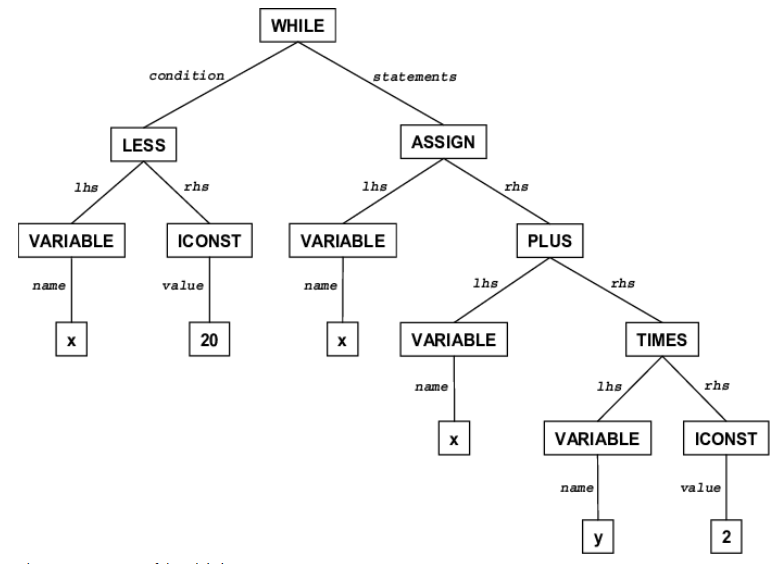
\includegraphics[scale=0.45]{../paper/res/WhileAST.PNG}
\end{figure}
\end{frame}

\begin{frame}{Kori\v{s}\v{c}eni alati}
    \begin{itemize}
        \item GumTree
        \item Eclipse JDT Core API
    \end{itemize}
\end{frame}

\begin{frame}[fragile]{Algoritam poredjenja}
    \begin{itemize}
        \item Pretpostavka: Semanti\v{c}ki ekvivalentni kodovi imaju iste vrednosti promenljivih na izlazu svakog bloka
    \end{itemize}
\begin{figure}[!h]
\centering
\begin{tabular}{ p{4.5cm} p{4.5cm} }
\begin{lstlisting}
int x = 1;
int foo()
{
    int a = 5;

    if (a > 3)
        x = 2;

    int c = 1;

    if (a > 3)
        c = 2;
}
\end{lstlisting}
&
\begin{lstlisting}
int y = 1;
int foo2()
{
    int a = 2;

    if (a < 3)
        y = 2;

    int c = 1;

    if (a < 3)
        c = 2;
}
\end{lstlisting}
\end{tabular}
\end{figure}
\end{frame}


\begin{frame}[fragile]{Algoritam poredjenja}
\begin{figure}[!h]
\centering
\begin{tabular}{ p{4.5cm} p{4.5cm} }
\begin{lstlisting}[basicstyle=\tiny\ttfamily]
// Block depth 0, ordinal 1
int x = 1;

int foo()
{
    // Block depth 1, ordinal 1
    // Vars passed: x = 1

    int a = 5;

    if (a > 3) {
        // Block depth 2, ordinal 1
        x = 2;
        // End of block: Update x in parent
    }

    // x = 2 here because of the update
\end{lstlisting}
&
\begin{lstlisting}[basicstyle=\tiny\ttfamily]
    int c = 1;
    if (a > 3) {
        // Block depth 2, ordinal 2
        c = 2;
        // End of block: Update c in parent
    }

    // Vars: x = 2, a = 5, c = 2
    // End of block: Update x in parent
}

// End of root block: x = 2
\end{lstlisting}
\end{tabular}
\end{figure}
\end{frame}


\begin{frame}[fragile]{Algoritam poredjenja}
\begin{figure}[!h]
\centering
\begin{tabular}{ | c | c | c |}
    \hline
    Block depth & Block ordinal & Variables \\
    \hline
    0 & 1 & x \\
    1 & 1 & x, a, c \\
    2 & 1 & x, a \\
    2 & 2 & x, a, c \\
    \hline
\end{tabular}
\end{figure}
\end{frame}



\begin{frame}[fragile]{Algoritam poredjenja}
\begin{figure}[!h]
\centering
\begin{tabular}{ p{4.5cm} p{4.5cm} }
\begin{lstlisting}[basicstyle=\tiny\ttfamily]
// Block depth 0, ordinal 1
int y = 1;  // Matches to x

int foo()
{
    // Block depth 1, ordinal 1
    // Vars passed: y = 1

    int a = 2;

    if (a < 3) {
        // Block depth 2, ordinal 1
        y = 2;
        // End of block: Update y in parent
    }

    // y = 2 here because of the update
\end{lstlisting}
&
\begin{lstlisting}[basicstyle=\tiny\ttfamily]
    int c = 1;
    if (a < 3) {
        // Block depth 2, ordinal 2
        c = 2;
        // End of block: Update c in parent
    }

    // Vars: y = 2, a = 2, c = 2
    // Conflict found: a = 5 in source, but found a = 2
    // End of block: Update y in parent
}

// End of root block: y = 2
\end{lstlisting}
\end{tabular}
\end{figure}
\end{frame}


\begin{frame}[fragile]{Algoritam poredjenja}
\begin{figure}[!h]
\centering
\begin{lstlisting}[basicstyle=\tiny\ttfamily]
Analyze(tree1: AST, tree2: AST)
begin
    if (CreateMatcher(tree1, tree2).OnlyUpdateActionsFound()):
        /* We have found only rename actions */
        print("Given snippets are equivallent")
        return

    /* In general case, traverse the first tree */
    vmap = tree1.TraverseAndRecordVars()

    /* Traverse the second tree and compare vars per block */
    conflicts = tree2.TraverseAndCompareVars(vmap)

    foreach (conflict in conflicts):
        print(conflict.Details)
end
\end{lstlisting}
\end{figure}
\end{frame}

\begin{frame}{Primeri}
    \centering
    :)
\end{frame}

\begin{frame}{Pobolj\v{s}anja}
    \begin{itemize}
        \item Pro\v{s}irivanje tipova na primitivne i referencne
        \item Simboli\v{c}ke promenljive
        \item Petlje sa poznatim brojem iteracija; razmotavanje
        \item Slo\v{z}eni konstrukti jezika - anonimne funkcije npr.
    \end{itemize}
\end{frame}



\begin{frame}{Pitanja}
    \centering
    ???
\end{frame}

\begin{frame}{}
    \centering
    Hvala na pa\v{z}nji!
\end{frame}

\end{document}
